\documentclass[11pt,a4paper,openany,oneside]{book}
\usepackage{preamble}
\usepackage{opstilling}
\usepackage{referencekommandoer}
\usepackage{pdfpages}

\author{Mikkel B. Goldschmidt \\ 3r, Nørre Gymnasium \\ SRP i matematik og fysik}

\usepackage{fancyhdr}
 
\pagestyle{fancy}
\fancyhf{}
\lhead{\leftmark \\ \rightmark}
\cfoot{\thepage}
\lfoot{Mikkel B. Goldschmidt}
\rfoot{3r, Nørre Gymnasium}






\title{Dæmpede svingninger og differentialligninger}
\begin{document}
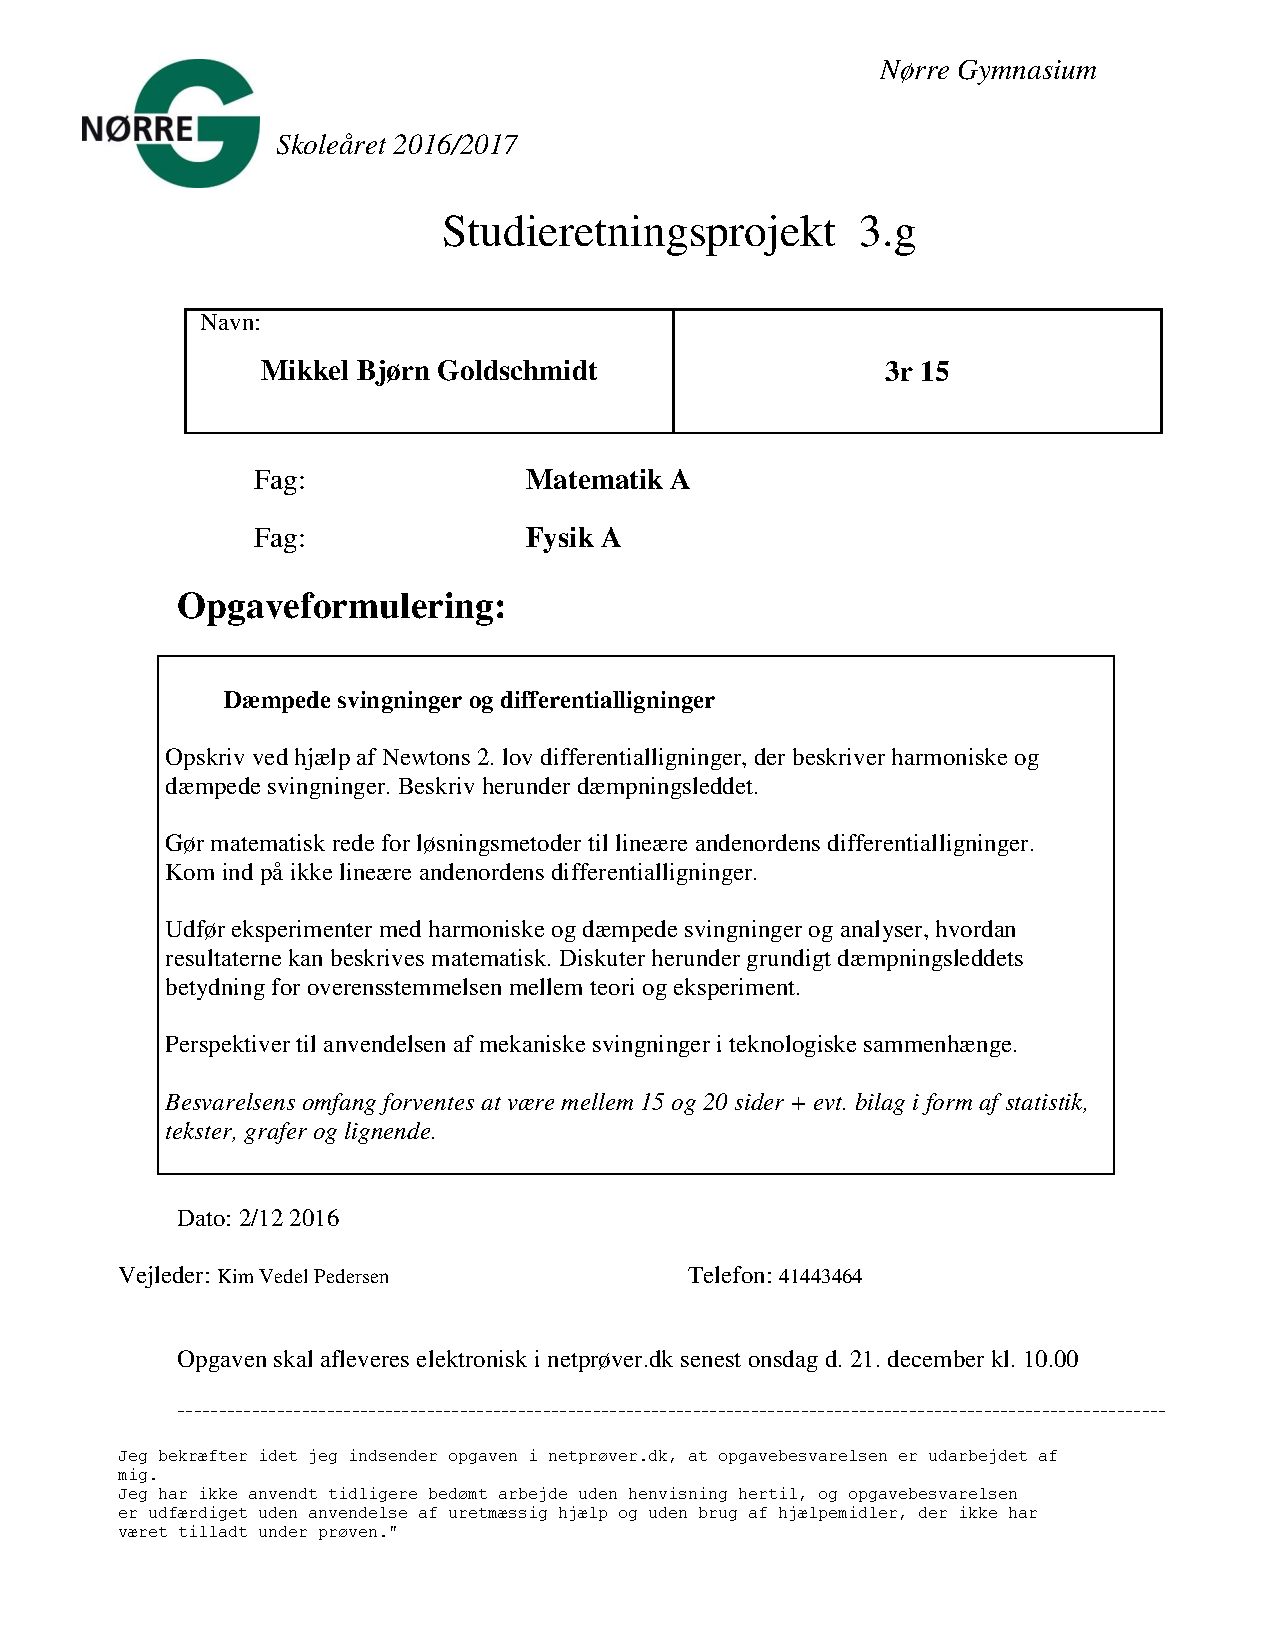
\includepdf[pages=1]{Forside.pdf}

\begin{titlepage}
	\centering
	
	{\scshape\LARGE Nørre Gymnasium\par}
	\vspace{1cm}
	{\scshape\Large SRP \\ \large Matematik og Fysik\par}
	\vspace{1.5cm}
	{\huge\bfseries Dæmpede svingninger og differentialligninger\par}
	\vspace{2cm}
	{\Large\itshape Mikkel B. Goldschmidt\par}
	
	
	\vfill
	vejleder\par
	Kim Vedel Pedersen
	\vfill

% Bottom of the page
	{\large Aflevering: 21. december 2016\par}
\end{titlepage}


\begin{singlespacing}
\tableofcontents
\end{singlespacing}
\pagebreak

\section*{Abstract}
\thispagestyle{plain}
This report examines the harmonic motion of a spring. 
It does this by examining the physical laws of springs and mechanical physics more broadly. 
These laws are then used to propose a mathematical model of the motion of an object hanging in a spring.

To easily solve these differential equations found in physics, this report examines them more generally. 
It describes the complete solution to the second order linear homogeneous differential equation, and gives a partial proof that the solution proposed is the complete solution. 

Having explained how to solve the differential equation, it then examines experiments meant to test whether the model of differential equations proposed about the motion are accurate.

Through two experiments it finds, that the second order linear homogeneous differential equation is a good description of the motion.
However, it also finds that the description is not perfect and then proposes an improvement of the model that makes the equations non-linear.
It argues why this improved model describes the motion better but it also shows why the model is a much harder mathematical problem to solve. 

The report then examines how this physical model can be used to describe parts a car suspension system.




\chapter{Introduktion af problemet}
Mange steder indenfor fysikken er svingninger helt centrale. 
De ses i alt fra lyd og musik, til broer som Tacoma bridge der gik i egensvingning. 
Dette gør at svingninger er et fænomen der er værd at studere for sig selv isoleret. 
Denne opgave kigger på den harmoniske svingning og på dæmpningen af denne.

Jeg vil tage udgangspunkt, i den bevægelse et lod har, når det hænges op i en fjeder og sættes i svingninger.

Jeg vil forsøge at opstille en matematisk differentialligningsmodel, der kan beskrive bevægelsen.
Dernæst vil jeg forsøge at bruge denne model, til at kunne beskrive direkte hvor loddet vil befinde sig til et bestemt tidspunkt. 
Dette vil kræve, at jeg kan løse de opsatte differentialligninger. 
For at finde denne løsning, vil jeg behandle problemet mere generelt ved brug af matematisk analyse. 

Jeg vil derefter udnytte de matematiske løsninger til at beskrive bevægelsen.
Disse modeller vil jeg da prøve af eksperimentelt, for at undersøge hvor godt de passer. 

Til sidst vil jeg kigge på, hvordan den teori jeg er kommet frem til, kan bruges til at analysere affjedringen af en bil. 
\vspace{1cm}

For at kunne lave denne opgave, vil der blive brug for noget baggrundteori både fra fysikken og matematikken. 
Denne er beskrevet nedenfor.



\section{Fysisk baggrundsteori}
\subsection{Hookes lov}\label{teori:Hooks lov}
Når man hiver i en fjeder, vil den have en kraft, modsatrettet den retning man hiver, der er proportional, med hvor meget man har strukket fjederen\refFysA{286}. 
Dette giver anledning til formlen 
$$F =k\cdot x$$
hvor $x$ er den længde, som fjederen er strukket, $F$ er kraften, som fjederen trækker med, og $k$ er proportionalitetskonstanten. 
$k$ kaldes i denne sammenhæng for fjederkonstanten.

\subsection{Newtons anden lov}\label{teori:Newtons anden lov}
Newtons anden lov fortæller ud fra den kraft et objekt påvirkes med og dets masse, hvor meget objektet vil accelerere. 
Den siger, at massen ganget med accelerationen af et objekt giver den kraft, som objektet bliver påvirket med\refFysA{217}.

\subsection{Vindmodstand}\label{teori:vindmodstand}
Når et objekt bevæger sig gennem luft eller en væske med en fart $v$, vil det have en gnidning med luften omkring sig, hvilket vil gøre farten mindre.
Ved et opslag i en formelsamling, ser man at kraften som vindmodstanden virker med, er proportional med farten i anden. 
Ved lav fart er dette dog næsten det samme som, at den er proportional med farten i første, og dette kan derfor være en okay antagelse af gøre sig i visse tilfælde\refMekanik{11}.

\section{Nødvendig matematisk baggrundsteori}
\subsection{Differentialligninger}
\newcommand{\LosEks}{$ \{ c\cdot e^{kx}|c\in \mR \} $}%Bruges i sætningen
Ved en differentialligning forstår vi en funktionnalligning, hvor funktionen minimum et sted er differentieret minimum en gang.
Ved en funktionalligning forstås en ligning, hvor det er en funktion, der er den ubekendte. 
Med en løsning til en differentialligning, refererer jeg fremover til en funktion, der gør differentialligningen sand. 
Ved den fuldstændige løsning til en differentialligning, refererer jeg fremover til mængden af \emph{alle} løsninger til differentialligningen. 
Nedenfor er et eksempel på en differentialligning. 
Denne er taget med både som eksempel og for at gøre udregninger mere tilgængelige senere.

\begin{thm}\label{thm:y'=k*y}
Lad $y$ være en differentialbel funktion og $k\in \mR$. Da har  differentialligningen $y' = ky$ den fuldstændige løsning \LosEks.
\end{thm}
\begin{proof}
Først vil jeg vise at alle funktioner i den påståede fuldstændige løsning er løsninger til differentialligningen.
Antag at $g$ er en funktion der ligger i \LosEks .
Da er $g=c\cdot e^{kx}$ for et eller andet reelt tal $c$.
Jeg indsætter da løsningen i ligningen: 

\begin{align*}
y' &= ky\\
g' &= kg\\
(c\cdot e^{kx})' &= k\cdot c\cdot e^{kx}\\
k\cdot c\cdot e^{kx} &= k\cdot c\cdot e^{kx}\\
\end{align*}
Jeg ser da, at de to sider er lig hinanden og dermed, at $g$ er en løsning. 

Nu vil jeg vise at hvis en funktion $h$ er en løsning til differentialligningen, da vil $h$ ligge i \LosEks.
Antag da netop at $h$ er en løsning til differentialligningen. 
Dermed ved vi, at $h'=k\cdot h$.
Jeg vil nu lave omskrivninger på denne ligning. 
For at gøre disse omskrivninger nemmere, vil jeg definere en funktion $s=e^{-kx}$, som vi ved at differentiere indser opfylder at $s'=k \cdot e^{-kx} = -ks$.
Ved omskrivning ses da:
\begin{align*}
h'&=k\cdot h \\
h'-kh &= 0\\
h's-ksh&=0 		& \text{(Ganger med }s\text{)}\\
h's+s'h&=0		& \text{(Ses ved $s'=-ks$)}\\
(hs)'&=0		&\text{(Ses ved kædereglen)}\\
hs+c_1 &= 0		&\text{(Ses ved at integrere, $c_1$ er integrationskonstant)}\\
h&= -c_1 \cdot \frac{1}{s}\\
h&= -c_1 \cdot e^{kx} &\text{(Ses ved $\frac{1}{s}=\frac{1}{e^{-kx}} = e^{kx}$)}
\end{align*}
Da ser vi at $h$ må være på formen en konstant ($-c_1$) ganget med $e^{kx}$, hvilet netop karakteriserer elementer i \LosEks. 
Dermed ligger $h$ i \LosEks.
Da er vist, at hvis en funktion er en løsning til differentialligningen, ligger den også i \LosEks og det er også vist, at hvis et element ligger i \LosEks da er det også en løsning. 
Dermed er \LosEks den fuldstændige løsning til differentialligningen. 
\end{proof}
\section{Forsøgsopsætning}\label{teori: opsatning af differentialligninger}
Hele denne opgave tager udgangspunkt i et forsøg.
I forsøget hænges et lod op i en fjeder der opfylder Hooks lov (se \ref{teori:Hooks lov}). 
Da tilføres loddet energi, således at det begynder at svinge. 
På figur \ref{fig:Basis Forsogsopsaetning} ses en skitse af forsøgets opsætning.

\begin{wrapfigure}{r}{0.4\textwidth}
\centering
\opstilling{-1}%Se opstilling.sty i hovedmappen for definition. Ser bedst ud med udgangsposition i -1.

\caption{Skitse af forsøgsopsætning.}
\label{fig:Basis Forsogsopsaetning}
\end{wrapfigure} 

\subsection{Teoretiske egenskaber for bevægelsen}
Man kan da overveje, hvilke kræfter der påvirker loddet. 
Det er klart at loddet er påvirket af en tyngdekraft. 
Derudover er loddet påvirket af kraften fra fjederen.
Til sidst vil loddets bevægelse også være påvirket af luften omkring den hvis loddet er sat i bevægelse. 
Jeg vil starte med at kigge på, hvordan loddet vil opføre sig hvis man ser på en forholdsvist langsom bevægelse i en kortere tidsperiode.
Da kan vi nemlig se bort fra luftens dæmpning. 

\subsubsection{Differentialligning uden dæmpning}\label{teori: Opstilling ligning uden dampning}
Hvis vi betragter nedadgående retning som værende positiv retning, kan vi altså opskrive den resulterende kraft på loddet som $F_{res} = -F_{fjeder}+F_{t}$, hvor $F_t$ betegner tyngdekraften på loddet. 
Vi bemærker dog at $F_t$ ikke er afhængig af af loddets stedfunktion. 
Dette gør den mere besværlig at arbejde med. 
Vi vil derfor sætte vores nulpunkt for kræfterne på en sådan måde at tyngdekraften bliver udlignet af at fjederen bliver strukket ud. 
Således har vi altså i stedet for $F_{res}=-F_{fjeder}$ eller $F_{res}+F_{fjeder}=0$.
Men vi kan da omskrive til en differentialligning ved at udnytte at $F_{fjeder}=k \cdot x(t)$ (se \ref{teori:Hooks lov}) hvor $x(t)$ er en funktion der beskriver loddets højde i forhold til et udgangspunkt (typisk vil dette udgangspunkt være den højde vil være i når det hænger stille).  
Derudover ved vi fra Newtons anden lov (se \ref{teori:Newtons anden lov}) at $F_{res}=m\cdot a(t) = m \cdot x''(t)$ 
(her er udnyttes at accelerationen af et objekt er lig dets stedfunktion differentieret dobbelt\refFysA{187}). 
Dermed får vi altså ligningen :
$$m\cdot x''(t)+k\cdot x(t)=0$$ 
som vi ser er en differentialligning i $x(t)$.

\subsubsection{Differentialligning med dæmpning}\label{teori: Opstilling af ligning med dampning}
Vi kan på samme måde som i forrige afsnit opskrive et udtryk der beskriver den resulterende kraft på loddet. 
Denne gang skal der bare trækkes et led mere fra på højresiden - nemlig luftmodstanden. 
Da vi i de fleste bevægelse tilnærmelsesvist kan beskrive luftmodstanden som værende proportional med hastigheden, kan vi skrive den som $- \mu x'(t)$ hvor $\mu$ er en proportionalitetskonstant og $x'(t)$ er stedfunktionen differentieret (og altså en beskrivelse af farten til tiden $t$\refFysA{187}).
her får vi altså en differentialligning på formen $m\cdot x''(t)=-k\cdot x(t)-\mu x'(t)$ eller omskrevet:
$$m\cdot x''(t)+\mu x'(t)+k\cdot x(t)=0$$
Fremover til $\mu x(t)$ blive omtalt som \textit{dæmpningsledet}, da det netop er luftmodstanden der gør at bevægelsen ikke bliver ved for evigt, da den giver anledning til en dæmpning. 

\chapter{Matematisk baggrund}
Før jeg undersøger, hvordan forsøget forventes at forløbe i teorien, bliver jeg nødt til at have noget mere matematisk baggrund. 
Det er denne matematiske baggrund, jeg vil forsøge at introducere i dette kapitel. 
Målet med hele kapitlet er, at kunne finde den fuldstændige løsning til den generelle lineære homogene andenordens differentialligning, samt at overveje hvad der sker, hvis dæmpningsledet i denne bliver i anden potens i stedet for i første. 
\section{Den komplekse eksponentialfunktion}
I gymnasiet bliver man kort introduceret til de komplekse tal, og jeg tager derfor for givet, at læseren kan løse en andengradsligning hvor diskriminanten er skarpt mindre end $0$ og derfor giver to komplekse løsninger. 
I gymnasiet lærer man dog ikke, at kunne opløfte tal i komplekse tal. 
Dette er dog en nødvendighed at kunne i denne opgave. 
Jeg vil derfor introducere definitionen af eksponentialfunktionen defineret på de komplekse tal $\mC$. 
Jeg vil ikke argumentere for, at denne opfører sig som den konventionelle definition med $\mR$, men bare lave en reference til en note fra DTU hvor dette kan ses. 

\begin{definition}[Den komplekse eksponentialfunktion]\label{def: Den komplekse eksponentialfunktion}

Lad $z=a+bi$ være et vilkårligt komplekst tal. Vi kalder da den komplekse eksponentialfunktion for $exp_\mC$. 
Vi definerer da denne til at være lig $exp_\mC (z)=e^{a} \cdot (cos(b) + sin(b)i)$.
Hvor $e$ er Eulers tal. 
\end{definition}

\begin{thm}\label{thm: expC = e^x}
$exp_\mC (x) = e^x$ hvis $x$ er et reelt tal. 
\end{thm}

\begin{proof}
Dette ses ret tydeligt ved at sætte $x+0i$ ind i definitionen af $exp_\mC$, der da vil blive $$exp_\mC(x) = e^x \cdot (cos(0)+sin(0)i)=e^x \cdot 1 = e^x \hspace{3cm}
\text{(Da $\sin (0)=0$ og $\cos (0)=1$)}$$
Dermed vist $exp_\mC (x) = e^x, \forall x \in \mR$
\end{proof}

\begin{thm}[Regneregler for $\exp_\mC$]\label{thm: regneregler for expC}
Følgende regneregler gælder for den komplekse eksponentialfunktion:
\begin{enumerate}
	\item $\eC (0)=1$
	\item $\eC (z_1+z_2) = \eC (z_1) \cdot \eC(z_2)$ for alle komplekse tal $z_1$ og $z_2$
	\item $(\eC (z))^n = exp_C (zn)$ for alle $n\in \mN$ og $z \in \mZ$.
\end{enumerate}
\end{thm}

\begin{proof}
Beviset for sætning \ref{thm: regneregler for expC} er ikke medtaget her grundet mangel på plads. Det kan læses i DTU's note om komplekse tal\refDTUKompleks{29.44}. 
\end{proof}

Vi kan se, at $\eC$ opfører sig på mange måder på samme måde som $e^x$, og specielt fordi $\eC$ altid tager de samme værdier som $e^x$ hvor den er defineret (de reelle tal, se sætning \ref{thm: expC = e^x}), tillader vi os fremover, at lade $e^x$ beskrive $\eC (x)$, og dermed er $e^x$ altså nu defineret fra $\mC$ over i $\mC$.
\section{Den andenordens lineære homogene differentialligning}
Det store problem i denne opgave er at bestemme den fuldstændige løsning til differentialligningerne, der er beskrevet i afsnit \ref{teori: opsatning af differentialligninger}.
Disse kan begge skrives på formen $y'' + by' + cy = 0$, hvor $b,c \in \mR$ og $y$ er en differentialbel funktion fra de reelle tal over i de reelle tal. 
Bemærk her, at der ikke er et konstantled foran $y''$. 
Dette gør ikke, at vi mister generalitet, da vi altid ville kunne dividere hele ligningen igennem med den konstant, der havde stået foran $y''$, og vi ville da have fået det på den ovenstående form. 
Jeg vil i dette afsnit bestemme den fuldstændige løsning til denne ligning. 
Mine udledninger her er stærkt inspirerede af Kalkulus\refKalkulus{529-539}. 

Jeg vil først vise et lemma, der vil gøre mine udregninger nemmere senere.

\begin{lemma}\label{thm: Summen af to losninger er en losning}
Hvis $g$ og $h$ er løsninger til den lineære andenordens differentialligning, da er $y(x) = C\cdot g(x) + D \cdot h(x)$ også en løsning for alle reelle konstanter $C,D$. 
\end{lemma}

\begin{proof}
Antag, at $h$ og $g$ er løsninger til den lineære andenordens differentialligning. 
Vi starter med at indse, at $y'=Cg' + Dh'$ og $y'' = Cg'' + Dh''$, ved brug af sumreglen for differentiation. 

Vi betragter da ligningen med $y$ indsat:
\begin{align*}
y'' + by' + cy 	&= (Cg'' + Dh'') + b(Cg' + Dh') + c(Ch + Dh)	& \text{(Egenskaberne beskrevet ovenfor)}\\
				&= Cg'' + Dh'' + bCg' + bDh' + cCh + cDh		& \text{(Ganger ind i parantes)}\\
				&= C(g'' + bg' + cg) + D(h'' + b'h + ch)		& \text{(Sætter udenfor parantes)}\\
				&= C\cdot 0 + D \cdot 0							& \text{(Udnytter at $g$ og $h$ er løsninger)}\\
				&= 0 
\end{align*}
Da kan vi se, at $y'' + by' + cy = 0$, dermed er $y$ en løsning til differentialligningen.
\end{proof}

Når vi snakker om lineære andenordens differentialligninger, er koefficienterne helt centrale for den fuldstændige løsning. 
Det vil vise sig senere, at en tilhørende andengradsligning til en lineær andenordens differentialligning, er helt central. Vi kalder denne for den \textit{karakterligningen}.

\begin{definition}[Karakterligningen]
Karakterligningen for en lineær homogen andenordens differentialligning $y'' + by' + cy = 0$, er ligningen $r^2 + br + c = 0$. 
Denne ligning har som bekendt en eller to komplekse løsninger (bemærk, at de reelle tal er indeholdt i de komplekse), $r_1 = \frac{-b + \sqrt{b^2 - 4c}}{2}$ og $r_2 = \frac{-b - \sqrt{b^2 - 4c}}{2}$.

Da andengradsligninger ofte er opstået ud fra polynomier, vil løsningerne til karakterligningen nogen gange blive refereret til som \textit{rødder}.
\end{definition}

Jeg vil i denne udledning kigge på to tilfælde af karakterligningen. 
Der hvor den har to komplekse løsninger, og der hvor den har to reelle.
Grunden til at jeg ikke kigger på, der hvor den har en reel rod, er, at det kræver, at $b^2 = 4c$ (da dette gør diskriminanten til $0$), hvilket er et særligt specialtilfælde, som meget sjældent vil forekomme i fysikken.

\subsection{To reelle løsninger af karakterligningen}
Jeg vil nu kigge på løsninger til den lineære andenordens differentialligning. 
Først indser jeg, at $e^{rx}$ er en løsning til den lineære andenordens differentialligning, hvis $r$ er en løsning til den karakterligningen.

\begin{thm}\label{thm: e^rx er en losning}
Lad en lineær andenordens differentialligning være på formen $y'' + by' + cy = 0$, og lad $r$ være en løsning til karakterligningen for denne.
Da er $e^{rx}$ en løsning til differentialligningen. 
\end{thm}

\begin{proof}
Jeg ser først på funktionen differentieret og dobbelt differentieret. 
Begge disse kan findes ved reglen for differentiation af den reelle eksponentialfunktion: 
$(e^{rx})' = r \cdot e^{rx}$ og 
$(e^{rx})'' = r\cdot (e^{rx})' = r^2 \cdot e^{rx}$.

Jeg indsætter nu funktionen i ligningen:
\begin{align*}
y'' + by' + cy 	&= (e^{rx})'' + b\cdot (e^{rx})' + c\cdot e^{rx} \\
				&= r^2 \cdot e^{rx} + br\cdot e^{rx} + c e^{rx} \\
				&= e^{rx} (r^2 + br + c)  & \text{(Sætter $e^{rx}$ udenfor parantes)}\\
				&= e^{rx} \cdot 0 		& \text{(Da $r$ er en løsning til karakterligningen)}\\
				&=0
\end{align*}

Da er vist, at $y=e^{rx}$ får differentialligningen til at blive $0$, og at dette derfor er en løsning. 
\end{proof}

\begin{thm}\label{thm: Den fuldstandige losning er en losning}
$y = C \cdot e^{r_1 x} + D \cdot e^{r_2 x}$ er en løsning til differentialligningen $y'' + by' + c = 0$ hvis $r_1$ og $r_2$ er reelle løsninger til dennes karakterligning, hvor $C,D$ er vilkårlige reelle tal.
\end{thm}
\begin{proof}
Vi ser først, at $e^{r_1 x}$ og $e^{r_2 x}$ begge hver for sig er løsninger ved brug af sætning \ref{thm: e^rx er en losning}.
Derefter kan vi bruge sætning \ref{thm: Summen af to losninger er en losning} til at se, at disse to løsninger ganget med vilkårlige konstanter også er en løsning.
Dermed må $y = C \cdot e^{r_1 x} + D \cdot e^{r_2 x}$ være en løsning til differentialligningen. 
\end{proof}

\begin{thm}[Den fuldstændige løsning]\label{thm: fuldstandig losning}
Den fuldstændige løsning til differentialligningen $y'' + by' + cy = 0$, med en karakterligning med to reelle løsninger $r_1$ og $r_2$ er mængden af alle funktioner på formen $C \cdot e^{r_1 x} + D \cdot e^{r_2 x}$, hvor $C,D$ er vilkårlige reelle konstanter.
\end{thm}
\begin{proof}
Det følger af sætning \ref{thm: Den fuldstandige losning er en losning}, at $y = C \cdot e^{r_1 x} + D \cdot e^{r_2 x}$ rent faktisk er en løsning. 
Da mangler jeg bare at vise, at hvis der eksisterer en løsning, så er den på netop denne form.

Først ses en egenskab omkring løsningerne i karakterligningen. 
Da vi ved at $r^2 + br + c$ har rødder $r_1$ og $r_2$, ved vi med algebraens fundamentalsætning (denne sætning er ikke vist i denne opgave, da det vil være for omfattende, men beviset kan ses i Kalkulus\refKalkulus{139-140}), at vi kan faktorisere ligningen sådan at: $r^2 + br + c = (r-r_1)(r - r_2) = r^2 -(r_1 + r_2)r + r_1 r_2$. 
Dermed kan vi se, at $r_1 + r_2 = -b$, da disse begge er koefficienter foran $r$ i hhv. første og sidste udtryk. 
Denne egenskab vil blive brugt imod slutningen af beviset. 

Vi antager at en funktion $f$ er en løsning til differentialligningen. 
Da vil jeg vise, at $f$ må være på formen $C \cdot e^{r_1 x} + D \cdot e^{r_2 x}$. 

Jeg introducerer en hjælpefunktion $u = \frac{f}{e^{r_1 x}}$. 
Ved omskrivning ses da $f = u \cdot e^{r_1 x}$. 
For at forsimple mine omskrivninger om lidt, vil jeg nu kigge på, hvordan $f'$ og $f''$ kan skrives ud fra $u$.
Alle følgende omskrivninger sker ved produktreglen (da både $u$ og $e^{r_1 x}$ er funktioner af $x$):
$$f' = (u e^{r_1 x})' = u'e^{r_1 x} + ur_1 e^{r_1 x}$$
$$f'' = (f')' = (u'e^{r_1 x} + ur_1 e^{r_1 x})' = u''e^{r_1 x} + 2\cdot u' r_1 e^{r_1 x} + u r_1^2 e^{r_1 x}$$

Da jeg ved, at $f$ er en løsning til differentialligningen, kan jeg opskrive differentialligninen og substituere $f, f'$ og $f''$, med de forskrifter som jeg har fået ved brug af $u$. 
\begin{align*}
0 	&= f'' + bf' + cf \\
	&= (u''e^{r_1 x} + 2\cdot u' r_1 e^{r_1 x} + u r_1^2 e^{r_1 x}) + b(u'e^{r_1 x} + ur_1 e^{r_1 x}) + c (u \cdot e^{r_1 x}) &\text{(Indsætter $f'$ og $f''$)}\\
	&= u''e^{r_1 x} + 2\cdot u' r_1 e^{r_1 x} + u r_1^2 e^{r_1 x} + bu'e^{r_1 x} + bur_1 e^{r_1 x} + cu \cdot e^{r_1 x}&\text{(Ganger ind i parantes)}\\
	&= u r_1^2 e^{r_1 x} + bur_1 e^{r_1 x} + cu \cdot e^{r_1 x} + u''e^{r_1 x} + 2\cdot u' r_1 e^{r_1 x} + bu'e^{r_1 x}  & \text{(Rokerer rundt på led)}\\
	&= ue^{r_1 x}(r_1^2  + br_1 + c) + u''e^{r_1 x} + 2\cdot u' r_1 e^{r_1 x} + bu'e^{r_1 x} & \text{($ue^{r_1 x}$ udenfor  parantes)}\\
	&= ue^{r_1 x} \cdot 0+ u''e^{r_1 x} + 2\cdot u' r_1 e^{r_1 x} + bu'e^{r_1 x} & \text{($r_1$ løser karakterligningen\footnotemark)}\\
	&= e^{r_1 x} (u'' + (2r_1 + b)u') & \text{(Sætter udenfor parantes)}\\
	&= u'' + (2r_1 + b)u' & \text{(Dividerer med $e^{r_1 x}$)}
\end{align*}
\footnotetext{$r_1$ er defineret til at være en løsning til karakterligningen, og derfor er $r_1^2 + br^1 + c = 0$}
Vi har da ligningen $u'' + (2r_1 + b)u' = 0$. 
Lad da en ny hjælpefunktion $h$ være defineret som $h = u'$. 
Da kan vi indsætte $h$ i den anden ligning og få:
$h' + (2r_1 + b)h = 0$. 
Dette er en differentialligning af første orden, som vi allerede har fundet en løsning på i sætning \ref{thm:y'=k*y}, 
hvor vi i dette tilfælde har $k = -(2r_1 + b)$.
Da har vi en fuldstændig løsning for $h$, nemlig $h=K \cdot e^{-(2r_1 + b)x}$, hvor $K$ er et vilkårligt reelt tal. 
Da kan vi ved at integrere $h$ finde $u$, dermed fås med normal integration af eksponentialfunktionen, at $u = \frac{K}{2r_1 + b} e^{-(2r_1 + b)x} + C$, hvor $C$ er integrationskonstanten. 
Vi ser, at $\frac{K}{2r_1 + b}$ er en reel konstant, som vi kan kalde $D$.
Da ved jeg også, at $f=u\cdot e^{r_1 x}$.
Jeg kan da, ved at indsætte min fundne værdi af $u$, finde en form på $f$:
\begin{align*}
f 	&= ue^{r_1 x}\\
	&= (D e^{-(2r_1 + b)x} + C)e^{r_1 x} &\text{(Indsætter $u$)}\\
	&= (D e^{-(2r_1 + b)x + r_1 x} + Ce^{r_1 x} &\text{(Ganger $e^{r_1 x}$ ind)}\\
	&= D \cdot e^{(-(2r_1 + b)+r_1)x} + C\cdot e^{r_1 x}&\text{(Flytter $x$ ud foran parantes)}\\
	&= D \cdot e^{(-r_1 - b)x} + C\cdot e^{r_1 x}\\
\end{align*}

Fra start så vi sammenhængen $r_1 + r_2 = -b$, og jeg kan derfor substituere $-b$ ind og få:
$$f(x) = D \cdot e^{(-r_1 +r_1 + r_2)x} + C\cdot e^{r_1 x}= D \cdot e^{r_2 x} + C\cdot e^{r_1 x} = C\cdot e^{r_1 x} + D \cdot e^{r_2 x}$$

Og da er det netop vist, at hvis $f$ er en løsning til differentialligningen, da er det også på formen $C\cdot e^{r_1 x} + D \cdot e^{r_2 x}$.
\end{proof}
\subsection{To komplekse rødder i karakterligningen}
Jeg vil ikke føre fuldstændigt bevis for den fuldstændige løsning, når løsningerne til karakterligningen er komplekse. 
Dette gør jeg ikke fordi at beviset minder meget om beviset for sætning \ref{thm: fuldstandig losning}.

Man kunne formode ud fra sætning \ref{thm: fuldstandig losning}, at løsningerne ville være på formen $C\cdot e^{r_1 x} + D \cdot e^{r_2 x}$.
Her bliver vi dog nødt til først at bemærke noget om $r_1$ og $r_2$.
Vi ved at disse to er løsninger til den samme andengradsligning, og dermed må de også være komplekst konjugerede af hinanden\refKalkulus{133}. 
Dermed må vi kunne skrive dem som $r_1 = a + bi$ og $r_2 = a-bi$. 
Man kunne derfor tænke, at løsningen til den lineære andenordens differentialligning ville være på formen $C\cdot e^{(a+bi) x} + D \cdot e^{(a-bi)x}$.
Dette kan vi dog skrive om med definition \ref{def: Den komplekse eksponentialfunktion} til $Ce^{ax}(\cos(bx) + \sin(bx) i) + De^{ax}(\cos(-bx) + \sin(-bx) i)$.
Vi kan da flytte $e^{a}$ udenfor parentes og få 
$e^{ax}(C(\cos(bx) + \sin(bx) i) + D(\cos(-bx) + \sin(-bx) i))$.
Da det gælder om cosinus og sinus at $\cos(-x)=\cos(x)$ og $\sin(-x)=-\sin(x)$, kan vi videre omskrive til 4
$e^{ax}(C(\cos(bx) + \sin(bx) i) + D(\cos(bx) - \sin(bx) i))$. 
Dette kan ved brug af additionsformlen for sinus omskrives videre til $e^{ax}\cdot \sqrt{C^2 + D^2}\sin(bx+\phi)$. 
Jeg vil ikke føre et argument for den sidste omskrivning.
Dette skyldes at der kræves en forholdvist dybdegående forståelse for de trigonometriske funktioner for at kunne gennemføre argumentet. 
Argumentet for omskrivningen kan ses i Kalkulus\refKalkulus{538-539}.

Man kan argumentere for at mængden af alle funktioner på den før omtalte form er den fuldstændige løsning til den lineære andenordens homogene differentialligning når den har komplekse rødder i sin karakterligning. 
Jeg vil dog udelade beviset, da det føres på næsten samme måde som beviset for sætning \ref{thm: fuldstandig losning}. 

Jeg har altså den fuldstændige løsning til differentialligningen (når rødderne er komplekse) som:
$y(x) = e^{ax}\sqrt{C^2 + D^2}\sin(bx+\phi)$, i fysiksammehænge sætter vi dog ofte $\sqrt{C^2 + D^2}$ til at være lig med en konstant $A$, da denne viser sig at være en amplitude. 
Vi har derfor løsningerne på formen:
$$y(x) = e^{ax}A\sin(bx+\phi)$$



\subsection{Den ikke-lineære andenordens homogene differentialligning}
I det vi indtil videre kun har kigget på den andenordens \textit{lineære} \textit{homogene} differentialligning, har vi lavet nogle antagelser som gør matematikken pæn, men disse holder dog ofte ikke i fysikkens verden.
Hvis man ser tilbage på afsnit \ref{teori:vindmodstand} om vindmodstand, har vi faktisk kun lavet matematisk teori der beskriver bevægelse ved lave hastigheder, da vi kun har kigget på når dæmpningsledet er i første. 
I afsnittet er det også beskrevet hvordan man ved høje hastigheder nærmere får at vindmodstanden er i anden.
Dette ville give anledning til en differentiallligning på formen:
$$y'' + b(y')^2 + cy = 0$$
Denne ligning er altså stadig homogen da den er lig med $0$, men ikke længere lineær. 
Det viser sig dog, at dette problem er markant sværere at løse end da dæmpningsledet var i første. 
Hvis vi kigger tilbage på beviset for sætning \ref{thm: fuldstandig losning}, så er det der fungerer i beviset at vi kan få hevet karakterligningen ud ved omskrivninger. 
Dette er kun muligt fordi alle tre led står i første. 
Havde vi forsøgt samme trick i den ikke-lineære, ville vi have fået en forkert potens på løsningen og dermed havde vi ikke kunnet nå i mål med beviset. 

Man kunne derfor prøve at løse den med et CAS-værktøj. 
Ved brug af Maple får jeg to løsninger (en med positivt og en med negativt fortegn, se $\pm$):
$$\int ^{y \left( x \right) }\!\pm 2\,{\frac {b}{\sqrt {4\,{{\rm e}^{-2\,b{
\it a}}}{\it C_1}\,{b}^{2}-4\,c{\it a}\,b+2\,c}}}{d{\it a}}-x-{
\it C_2}=0 \text{ hvor } C_1,C_2 \in \mR
$$
Dette har vi ikke redskaberne til at forstå med gymnasiepensum. 
For så vidt giver integralet og de to konstanter mening, men det at der kun er en øvre grænse og at grænsen er den funktion vi forsøger at finde, gør at dette nok ikke er en farbar vej til til at finde en løsning. 

Derfor er der nok kun vejen frem at løse problemet numerisk. 
Ved en numerisk løsning af en differentialligning, forstås at man kender en værdi på grafen og beregner flere værdier ud derfra.
Dog skal man når man regner på andenordens differentialligninger kende en sammenhørende værdi af $y$, $y'$ eller $y''$ for at kunne give et entydigt svar\refKalkulus{539}.
Jeg vil forsøge at lave en numerisk løsning senere, når jeg skal behandle data fra mine forsøg. 


\chapter{Forsøg}
Hele denne opgave tager udgangspunkt i et forsøg.
Jeg vil her beskrive dette forsøg, og udnytte den matematik, jeg har beskrevet, til at finde ud af om de opstillede differentialligninger fra afsnit \ref{teori: opsatning af differentialligninger} rent faktisk passer på virkeligheden.

Jeg har udført to forsøg, som hvert i sær er tænkt til at afprøve et stykke teori:
\begin{itemize}
	\item Svingning af lod i luft i kort tid
	\item Svingning af lod i luft i længere tid
\end{itemize}

Det første forsøg er ment til at skulle passe på differentialligningen uden dæmpningsled.

Det andet forsøg er tænkt til at passe med et dæmpningsled ved lav hastighed, og altså derfor med dæmpningsledet i 1. potens.
Dette forsøg undersøger også om en model med dæmpningsledet i anden potens vil fungere bedre, end en med leddet i første potens.  

\section{Forsøg: Svingning af lod i luft i kort tid}

\subsection{Forsøgsbeskrivelse}

\subsection{Hypotese}

\subsection{Databehandling}

\subsection{Konklusion}



\section{Forsøg: Svingning af lod i luft i længere tid}

\subsection{Forsøgsbeskrivelse}
Dette forsøg forløber nøjagtigt på samme måde som forsøg 1 (se forsøgsbeskrivelse \ref{exp1: Beskrivelse af experiment}).
Der er dog den forskel at forsøget forløber over $50$ sekunder og at forsøget kun er gentaget 5 gange. 

Jeg gør brug af samme fjeder og lod som i forsøg 1.

\subsection{Hypotese}
Da dette forsøg forløber over længere tid end det forrige forsøg, forventes det at vindmodstanden vil spille en markant rolle. 
Derfor vil vi forvente at det følger en anden differentialligning hvor dæmpningsledet er med, nemlig:
$m\cdot x''= -\mu \cdot x' - k\cdot x$
eller omskrevet til den form som vi har behandlet matematisk:
$$x''+ \frac{\mu}{m} \cdot x' + \frac{k}{m}\cdot x=0$$
Dette kan vi  se er en andenordens homogen lineær differentialligning.
Vi kan derfor opskrive en karakterligning for den:
$r^2 + \frac{\mu}{m} r + \frac{k}{m} = 0$, med rødderne $r = \dfrac{-\frac{\mu}{m} \pm \sqrt{\frac{\mu^2}{m^2}-4\frac{k}{m}}}{2}=
-\frac{\mu}{2m}  \pm   \frac{\sqrt{-\frac{\mu^2}{m^2}+4\frac{k}{m}}}{2}$.
Vi vil nu gerne bruge disse rødder til at opskrive en forventet funktion til beskrivelse af bevægelsen. 
Dog har vi det problem at vi ikke ved om rødderne bliver komplekse eller reelle, da dette afhænger af hvor stor en værdi $\mu$ er i forhold til $k$.
Hvis vi har at størrelsen $\frac{\mu^2}{m^2}-4\frac{k}{m}$ er positiv, så må vi have reelle rødder, hvorimod vi må have komplekse hvis den er negativ. 
Der er selvfølgelig også grænsetilfældet hvor det er lig $0$, men da dette er højest usandsynligt vil jeg ikke behandle dette. 

Da vi skal opstille en hypotese, vil det være forventeligt at rødderne er komplekse. 
Dette fordi vi i forsøg 1 gjorde præcis det samme som her og så at en model med komplekse rødder så ud til at fungere. 

I det vores løsninger til karakterligningen forventes at være komplekse, kan vi da forvente en bevægelse der kan beskrives ved:
$$e^{-\frac{\mu}{2m} \cdot x}A\sin(\frac{\sqrt{-\frac{\mu^2}{m^2}+4\frac{k}{m}}}{2} \cdot x+\phi)$$
\subsection{Data}
Rådata til dette forsøg er vedlagt i filen ''Forsøg 2 - Data.pdf'' og data til bestemmelse af fjederkonstanten ligger i filen ''Forsøg 1 og 2 fjederkonstant - Data.pdf''. 


\subsection{Databehandling}

\subsection{Konklusion}



\section{Opsummering af forsøg 1 og 2}
I både forsøg 1 og 2 har det være muligt at bruge den andenordens lineære homogene differentialligningsmodel til at beskrive bevægelsen. 
Det viser sig, at den tid som loddet svinger, er det, der betyder mest for, om dæmpningsledet skal tages i betragtning. 
Det viser sig også, at tiden lodet svinger har betydning for, om modellen kan bruges. 
Ved de forholdsvis lave amplituder, som jeg har studeret i forsøg 2, har det vist sig, at modellen bliver for upræcis efter ca. 40 sekunder. 

Hvis modellen skal kunne bruges over en længere tidsperiode, bliver man nødt til at bruge en numerisk løsning af den ikke-lineære model, som er beskrevet tidligere.
I denne forbindelse vil det være optimalt at bestemme $\mu$ ud fra mere specifik teori om vindmodstand, da størrelsen ikke ser ud til at kunne bestemmes entydigt ud fra disse forsøg - grundet de varierende værdier af $a$ i tabel \ref{tabel: best fit exp2}.

Dog er modellen meget præcis og får lave afvigelser eksperimentelt, derfor ser differentialligningerne ud til at være et stærkt værktøj til at beskrive modellen. 


\chapter{Sammenfatning og konklusion}
Efter at have undersøgt den harmoniske svingning teoretisk, har det været muligt for mig at opsætte en model til at beskrive bevægelsen. 
Denne model gav anledning til matematiske problemstillinger, som ikke har været behandlet i gymnasiet.
Mere specifikt fik jeg brug for at kunne løse en andenordens lineær homogen differentialligning. 
Dette problem behandlede jeg matematisk, og jeg fandt frem til en fuldstændig løsning for differentialligningen, som jeg delvist fik givet et bevis for. 
Med denne løsning lykkedes det mig at kunne lave en stedfunktion ud fra min differentialligningsmodel.
Jeg udførte så eksperimenter, der skulle undersøge, hvor godt denne stedfunktion (og dermed også differentialligningen fra min model) passede.
Det viste sig, at modellen passede ganske godt på det, jeg observerede.
Dog var der mindre problemer med modellen, som jeg undersøgte og løste ved at finde en model, som passede bedre i fysikken, men som dog var et væsentligt mere udfordrende matematisk problem.

Det er altså lykkedes mig at beskrive den harmonisk dæmpede svingning med en forholdsvis god fysisk model ved hjælp af matematisk analyse af en differentialligningsmodel.
 
Af videre arbejde ville det være godt at kunne studere den forbedrede model og se, om der kan findes måder at beskrive den nemmere matematisk. 

\chapter{Perspektivering - Affjedring af biler}
Den harmoniske svingning optræder mange andre steder i mekanikken, end bare når et lod svinger i en fjeder.
Den ses blandt andet i forbindelse med penduler og generelt med ting, der drejer rundt.
Derudover er det også relevant at kigge på i forbindelse med større bygninger, eksempelvis broer, der kan gå i svingninger hvis de ikke er konstrueret rigtigt. 

Et andet sted hvor man kan se svingninger af fjedre meget markant, er i forbindelse med affjedring af biler. 
Det er nemlig sådan at en bils hjul er forbundet til fjedre. 
En skitse af dette kan ses på figur \ref{fig: Affjedring af bil}.

\begin{wrapfigure}{r}{0.4\textwidth}
\center
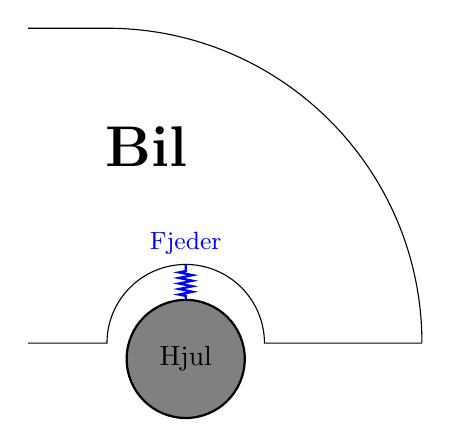
\begin{tikzpicture}
\tikzstyle{spring}=[thick,decorate,decoration={zigzag,pre length=0.05cm,post length=0.05cm,segment length=2}]

\draw (-2,0)--(-1,0)--(-1,0) arc [radius=1, start angle=180, end angle= 0]--(1,0)--(3,0);%Bund af bil uden hjul

\draw (3,0) arc [radius=4, start angle=0, end angle = 90] -- (-2,4) ;%Top af bil

\draw[fill=gray, thick] (0,-0.2) circle (0.75) node {Hjul};%hjulet
\node at (-0.5,2.5) {\huge \textbf{Bil}};
\draw[spring, blue] (0,0.55)--(0,1) node[above, blue] {\small Fjeder};

\end{tikzpicture}
\caption{Skitsetegning af fjeder (blå) fastsat til bils hjul.}
\label{fig: Affjedring af bil}
\end{wrapfigure}

Fjederen er til for at sørge for, at bilen hele tiden fastholder kontakt med vejen - også selvom den kører over en ujævnhed. 
Hvis fjederen går i stykker, kan det være meget problematisk. 
Der kan ske det, at fjederen dæmper for langsomt, og at man derfor oplever at bilen hopper.
En video af af dette kan ses på YouTube\refBilVideo.
På videoen ser vi en mand, der trykker på forenden af sin bil. 
Når han giver slip, står bilen og svinger op og ned. 
Hvis man betragter denne svingning med den teori, der er beskrevet i denne opgave, så svarer bilen til vores lod.
Vi er da interesserede i at få svingningen af bilen til at dø ud så hurtigt som muligt. 
Her arbejder vi ikke med luftmodstand, men derimod med en mekanisk dæmpning. 
Hvis vi antager, at svingningen dæmpes på en måde, således at dæmpningen er proportional med hastigheden af svingningen med en proportionalitetskonstant $\xi$, har vi igen en lineær andenordens homogen differentialligning

$$mx''(t)+\xi x'(t) + k x(t) = 0$$

hvor $k$ er fjederkonstanten for bilens fjeder, $m$ er bilens masse, og $x$ er en funktion af tiden, der beskriver, hvor højt/lavt bilen befinder sig i forhold til sit udgangspunkt.

Da vi er interesserede i, at bilen hopper så lidt som muligt, er vi ikke interesserede i en harmonisk svingning. 
Vi ved fra teorien tidligere, at der opstår en harmonisk svingning, når rødderne i karakterligningen er komplekse. 
Derfor er man interesseret i at få en god nok kombination af dæmpningskonstant og fjederkonstant til, at rødderne i karakterligningen ikke bliver komplekse. 

Vi vil derfor gerne prøve at kigge på karakterligningen. 
Vi får da en ligning $mr^2 + \xi r + k = 0$ hvilket giver os løsningerne (med andengradslignings løsningsformel):

$$r = \dfrac{-\xi \pm \sqrt{\xi ^2 - 4mk}}{2m}$$

For at vi ikke får komplekse rødder, skal vi altså have, at størrelsen $\xi ^2 -4mk$ er ikke-negativ, og det skal altså gælde at $0 \leq \xi ^2 -4mk $ eller omskrevet at $4mk \leq \xi ^2 $.
Her fra er man dog nødt til at vide mere omkring biler og kunne foretage nogle eksperimenter for at kunne fortsætte. 
Vi ved nemlig intet om $\xi$, og om hvordan dæmpning skabes. 

I forhold til videoen, kan vi se at bilen lige pludselig svinger, og at karakterligningen derfor må have komplekse løsninger.
Vi ved derfor, at der er sket en ændring af $k,m$ og $\xi$ sådan, at det ikke længere gælder, at $4mk \leq \xi ^2 $.
Da bilens masse, $m$, formentlig ikke har ændret sig, må vi altså enten have at $k$ er blevet større eller at $\xi$ er blevet mindre. 
Oversat til fysik, har vi altså enten, at fjederen er blevet mere hård og derfor har en højere fjederkonstant, eller at dæmpningssystemet ikke fungerer som det skal.

\vspace{0.75cm}

Bemærk, at dette ikke på nogen måde er baseret eksperimentelt    på biler, men bare er et forsøg på at overføre min model fra loddet til en bil. 
Det er mange ting, der bør tages højde for, som denne perspektivering ikke kigger på.
Dog kan det ses at modellen, som der er fundet frem til i denne opgave, ikke er irrelevant til at beskrive andre fysiske fænomener.



\begin{thebibliography}{9}

%\bibitem{Bog_hele bogen}
%  Forfatter,
%  (Årstal, s. ...). 
%  Titel (Udgave). 
%  By,
%  Forlag

 
\bibitem{FysikA}
  Knud Erik Nielsen og Esper Fogh,
  (2011, s. \textbf{???Tjek efter???}). 
  Vejen til fysik A2 (2. udgave). 
  Silkeborg,
  Forlaget Hax

\bibitem{Mekanik}
  Gunnar Christiansen, Erik Both og Preben Østergaard Sørensen,
  (2002, s. "9-11'' - "9-22"). 
  Mekanik. 
  Lyngby,
  Stougaard Jensen/Albertlund
  
\bibitem{DTU-Kompleks}
(11. december 2016, Sætning 29.44), Komplekse tal. Hentet fra:
\url{http://01005.mat.dtu.dk/materialer/enoter/afsnit/NUID43-tn29/}

\bibitem{Kalkulus}
  Tom Lindstrøm,
  (2006, s. 529-541). 
  Kalkulus (3. udgave). 
  Oslo,
  Universitetsforlaget
  
  
\end{thebibliography}
\section*{Bilagsliste}
Dette er en liste over alle vedlagte bilag samt en kort beskrivelse af dem.
Bemærk at specielt rådata til forsøgene er meget lange dokumenter og derfor ikke bør printes. 

\begin{itemize}[leftmargin=0.5\textwidth]
	\item[\textbf{Forsøg 1 - Data.pdf}:] Rådata fra forsøg 1 med svingning af lod i kort tid. ($130$ sider)
	\item[\textbf{Forsøg 2 - Data.pdf}:] Rådata fra forsøg 2 med svingning af lod i længere tid. ($255$ sider) 
	\item[\textbf{Forsøg 1 og 2 fjederkonstant - Data.pdf}:] Rådata til bestemmelse af fjederkonstanten for den fjeder der blev benyttet i forsøg 1 og 2. ($1$ side)
	\item[\textbf{Forsøg 1 - grafer.pdf}:] Grafer med data samt best-fit-kurver for forsøg 1. ($12$ sider)
	\item[\textbf{Forsøg 2 - grafer.pdf}:] Grafer med data samt best-fit-kurver for forsøg 2. ($6$ sider)
\end{itemize}


\end{document}
